\documentclass{article}
\usepackage{graphicx} % Required for inserting images
\usepackage{tikz}
\usepackage[left=1cm,right=1cm,top=1cm,bottom=1cm]{geometry}
\usepackage{hyperref}
\hypersetup{
    colorlinks=true,
    linkcolor=blue,
    filecolor=magenta,      
    urlcolor=cyan,
    }

\title{Physik - Zusammenfassung fürs Abitur}
\author{Maximilian Penke, Emil Maihorn}
\date{January 2024}

\renewcommand*\contentsname{Gliederung}

\begin{document}

    \maketitle

    \begin{abstract}
        Dies ist eine Zusammenfassung für die Inhalte des Berliner Abiturs von 2024 im Fach Physik. Dabei ist des in die vier Halbjahre unterteilt, wobei es jeweils Differenzierungen gibt. Dafür werden die Inhalte der Einzelthemen erklärt, mit der allgemeinen Umsetzungsweise versehen und darauf folgend mit unterschiedlichen Beispielen veranschaulicht.
    \end{abstract}

    \tableofcontents

    \section{Allgemeine Hinweise zur Notation}

        \subsection{Koordinatensysteme} 
        mehr unter \href{https://gcm.schule/material/2023/physik/lk12/01_Koordinatensysteme_Felder.md}{material}
        
        Zu beachten:
        \begin{itemize}
            \item Die Pfeile an der x- und y-Achse und die x- und y- Achsenbeschriftung
            \item Die Kennzeichnung des Koordinatenursprungs und die x- und y-Achseneinteilung
            \item Die Einzeichnung eines Punktes mit einem Kreuz
            \item Punktkennzeichnung mit der Beschreibung
        \end{itemize}

        \begin{figure}[h]
            \centering
            \begin{tikzpicture}[x=1cm, y=1cm]
                % Axes
                \draw [->] (0,0) -- (3,0) node [right] {x [Physikalische Einheit] };
                \draw [->] (0,0) -- (0,3) node [left] {y [Physikalische Einheit]};
                \draw [-] (0,0) -- (-3,0) node [right] {};
                \draw [-] (0,0) -- (0,-3) node [left] {};
            
                \draw [-] (-0.1, -0.1) -- (0.1,0.1);
                \node [below] at (-0.2,0) {0};
                \draw [-] (1, -0.1) -- (1,0.1);
                \node [below] at (1,-0.1) {1};
                \draw [-] (-0.1, 1) -- (0.1,1);
                \node [left] at (-0.2,1) {1};
                \draw [-] (1.5, 1.4) -- (1.4,1.5);
                \draw [-] (1.4, 1.4) -- (1.5,1.5);
                \node [above] at (1.5,1.5) {$P(1.45|1.45)$};
            \end{tikzpicture}
        \end{figure}

        Beispiel:

        \begin{figure}[h]
        \centering
        \begin{tikzpicture}[x=1cm, y=1cm]
            % Axes
            \draw [->] (0,0) -- (3,0) node [right] {t [s] };
            \draw [->] (0,0) -- (0,3) node [left] {U [V]};
            \draw [-] (0,0) -- (-3,0) node [right] {};
            \draw [-] (0,0) -- (0,-3) node [left] {};
        
            \draw [-] (-0.1, -0.1) -- (0.1,0.1);
            \node [below] at (-0.2,0) {0};
            \draw [-] (1, -0.1) -- (1,0.1);
            \node [below] at (1,-0.1) {1};
            \draw [-] (-0.1, 1) -- (0.1,1);
            \node [left] at (-0.2,1) {1};
            \draw [-] (1.5, 1.4) -- (1.4,1.5);
            \draw [-] (1.4, 1.4) -- (1.5,1.5);
            \node [above] at (1.5,1.5) {$P(1.45s|1.45V)$};
        \end{tikzpicture}
    \end{figure}
        
    \newpage
        \subsection{Felder skizzieren}
        
            Zu beachten:
            \begin{enumerate}
                \item Feldlinien sind Vektoren
                \item Der Schwanz von Feldlinien beginnt stets am Ursprung
                \item Feldlinien werden mit gleichem Abstand zueinander gezeichnet, wenn das Feld homogen ist.
                \item Je dichter die Feldlinien, desto stärker das Feld.
            \end{enumerate}

        \subsection{Schaltkreise und Versuchsaufbauten}

        \subsection{Notation in der Rechnung}

            Geg, Ges und Lös sind nicht Pflicht aber hilfreich! \\
            Einheitenumrechnung ist ebenfalls nicht Pflicht, aber eine sehr gute Methode, um die Korrektheit der Antwort zu überprüfen. Diese kann in einer Nebenrechnung vollzogen werden. \\
            Generell gilt: stets in 10er-Potenzen umformen und damit rechnen! \\
            Regeln zur Potenzumformung: $10^m \cdot 10^n = 10^{m+n}$, $\frac{10^m}{m^n} = 10^{m-n}$ \\
            Stets bedenken: Aus Subtraktionen und Summen kürzen nur die Dummen! \\

    \section{Q1: Graviattion}

        \href{https://gcm.schule/material/2023/physik/lk12/index_Q1.md}{Material}

        \subsection{Einführung in Felder}
            In der Physik werden Felder genutzt, um Kräfte, Flüsse und Bewegungen zu beschreiben.
            Die Felder, die für uns wichtig sind, sind sog. Vektorfelder der Elektromagnetischen Kraft
            und der Gravitationskraft. \\
            In der Physik werden Kräfte zwischen zwei Objekten gerne mit Vektoren beschrieben. Ungefähr so:
            \begin{figure}[h] \label{figure3: Gravitationskraft} 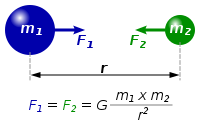
\includegraphics{graphics/universalGravitation.png}\end{figure}   
            Die Massen $m_1$ und $ m_2 $ ziehen sich durch Gravitation an.
        \subsection{Darstellung von Feldern}


        \subsection{Impulserhaltungssatz}
        
        \subsection{Gravitation}
        
        	\paragraph{Einführung \newline}
        	
        		Gravitationskraft beschreibt eine Kraft zwischen zwei Massen. Gravitationskraft nimmt mit großerer entfernung der Massen ab und Lässt sich im gegensatz zu Maget- und Elektrischenfeldern abschirmen. Im Raum lässt ein Gravitationsfeld Kraft auf Massen wirken. Dieses Feld geht von Massen aus.
        
         	\subsubsection{Kosmische Geschwindigkeiten}
         		
         		\paragraph{1. Kosmische Geschwindigkeit \newline}
         		
         			Die erste Kosmische geschwindigkeit beschribt die nötige Geschwindigkeit welche ein Körper haben muss um in seiner Kreisförmigen Umlaufbahn zu bleiben. Sie lässt sich aus der gleichsetzung der Zentripitalkraft und dem Gesetz Universellen Gravitation herleiten. 
         			
         			\[v_{k_{1}} = \sqrt{\frac{G \cdot M} {r}}\]
         			
         		\paragraph{2. Kosmische Geschwindigkeit \newline}
         		
         			Die zweite Kosmischegeschwindigkeit beschreibt die nötige Geschwindigkeit um aus dem Gravitationsfeld einer Masse zu entkommen. Sie lässt sich 
         			
         			\[Arbeit im Graviatationsfeld \longrightarrow W_{G} = f_{G} \cdot r\]
         			
         			\[ umstellen nach v  \longrightarrow W_{g} = E_{Kin} = \frac{1}{2} m \cdot v ^2 = f_{g} \cdot r\]
         			
         			\[v_{k_{2}} = \sqrt{\frac{2\cdot G \cdot M} {r}}\]
         			
        
            \subsubsection{Keplersche Gesetze}
            
            	\paragraph{1. Keplersche Gesetz \newline}
            		
            		Die Bahn eines Jeden Planeten ist Elliptisch in einem der Brennpunkte steht die Sonne.
            		
            	\paragraph{2. Keplersche Gesetz \newline}
            	
            		Die Geschwindigkeit der Planeten, auf hre Bahnelipse, variieren so, das eine von der Sonne zum Planeten gezogener Fahstrahl, in gleichen zeiten gleiche Flächen überstreift. 
            		
          		\paragraph{3. Keplersche Gesetz \newline}
          		
          			
          			
        
        	\subsection{Gravitationskraft und Berechnung}
        
        \subsection{Elektrisches Feld}
        
        	\paragraph{Einführung \newline}
        	
        		Elektrischefelder sind Felder welche eine Kraftwirkung auf Ladungen und Geledene Teilchen haben. Sie gehen von Geledenen Teilchen und Ladungen aus. Es gibt Positive sowie Negative Ladungen. Gleiche Ladungen stoßen sich gegenseitig ab. Unterschiedliche Ladungen ziehen sich gegenseitig an. 
        		
       		\paragraph{Elektrisches Potential}
       		
       			Potentiale sind eigenschaften eines Feldes welche die Wirkung des Felds auf Jeglichen Ladung beschreiben. Damit beschreibt es die Sträke des Feldes an einem Bestimmten Ort.
       			Equipotential ebene beschreibt die Ebene glechen Potentials in dem Feld. Aus diesem Grund ist eine verschiebung einer Ladung in einer Equipotentialebene Energetisch "Kostenlos". 
        
        	\subsubsection{Kondensatoren}
        	
        		\paragraph{Einführung \newline}
        		
        			Ein Kondensator ist eine methode mit welcher Energie in einem Elektrischen Feld gespeichert wird. Das Elektrische Feld wird im Kondensatror aufgebaut indem Spannungen zwischen den beiden Kondensatorplatten aufgebaut werden und sich die Ladungen zu den Kondensatorplatten bewegen. 
        			
       			\paragraph{Physikalische Größen}
       			
       				\subparagraph{Kapazität - C}
       				
       					Die Kapazität gibt die menge der Ladungen an, welche Gespeichert werden können. 
       					
       					\[C = \frac{Q}{U} = [f] = [\frac{A\cdot s}{V}]\]
     					
     				\subparagraph{Elektrische Feldstärke}
     				
     					Sie beschreibt die Kraft welche auf Jegliche Ladung zwischen den Kondensatorplatten wirkt. 
     					
     					\[im Kondensator \longrightarrow E = \frac{U}{d}\] 
     					\[Allgemein \longrightarrow E = \frac{F}{Q}\]
     					
    				\subparagraph{Kapaziziven Wiederstand}
    				
    					Im Gleichstromkreis wirkt der Konensator wie ein Wiederstand. Der Wiederstand ist Unendlichhoch das kein Strom fließen kann. 
    					
    				\subparagraph{Durchschlagsfestigkeit}
    				
    					Die Durchschlagsfestig ist eine Eigenshaft des Isolator zwischen den Kondensatorplatten ab welchem ein Ladungsdurchschlag stattfindet. Sie wird Experimentell ermittelt. 
    					
    					\[E_{d} = \frac{U_{d}}{d}\]
    					
    				\subparagraph{Aufladen eines Kondensators}
    				
    					Das Aufladen eines Kondensators nähert sich Asymthotisch eines Spannung, da sich an dem Kondensatorplatten Ladungen sammeln und somit ein Wiederstand für das Erhöhen der Ladungsmenge, weshalb sich dies Aysmthotisch verhält. 
    					
    				\subparagraph{Spannung}
    				
    					Die Spannung beschreibt die Differenz zwischen zwei Ladungen. 
    					
    					\[Fuer Homogene Felder \longrightarrow U = \Delta \phi = \phi_{1} - \phi_{2}\] 
    					\[Fuer inhomogene Felder \longrightarrow U = \]
    					
       			
       			\paragraph{Verhalten in Schaltungen}
       			
       			
       				\subparagraph{Capazität in Reihe}
       					
       					Der Kehrwert der Gasamt Kapazität ist die Summe der Kerhwerte der Kapazitäten. 
       					
       					\[ \frac{1}{C} = \frac{1}{C_{1}} + \frac{1}{C_{2}} + ... + \frac{1}{C_{n}}\]
       					
       					Falls man die  Kapazität eines Systems erhöhen möchte muss man Kondensatoren Parralel Schalten. 
       					
       				\subparagraph{Spannung in Reihe}
       					
       					Die gesamt Spannung der in einem in Reiche geschalteten Kondensator Konstruckt entsprichte der Summe der einzel Kondensatoren. 
       					
       					\[U = U_{1} + U_{2} + ... + U_{n}\]
       					
       				\subparagraph{Kapazität in Parallel}
       				
       					Die gesamt Kapazität eines Kondensatorsystems ist die Summe aller einzel Kondensatoren
       					
       					\[C = C_{1} + C_{2} + ... + C_{n}\]
       					
       				\subparagraph{Spannung  in Parallel}
       				
       					Die gesamt Spannung ist gleich der einzel Spannung der Kondensatoren
       					
       					\[U = U_{1} = U_{2} = ... = U_{n}\]
        
        \subsection{Magnetisches Feld}

    \section{Q2: Elektromagnetische Wellen}

    \href{https://gcm.schule/material/2023/physik/lk12/#q1}{Material}
    	\subsection{Elektromagnetische Induktion}
    	
    	\subsection{Wahlgebiet Wechselstrom}
    	
    		\subsubsection{Phasenverschiebung}
    		
    		\subsubsection{Wiederstände (Ohmscher, Kapazitiver und Induktiver)}
    		
    		\subsubsection{Scheinwieerstand bei einer Reichenschaltung von pohmschen, kapazitivem und induktivem Wiederstand}
    	
    	\subsection{Elektromagnetische Schwingungen}

    \section{Q3: Quantenphysik}

    \href{https://gcm.schule/material/2022/physik/lk13/}{Material}
    
    	\subsection{Ladungsträger in elektrischen und magnetischen Feldern}
    	
    	\subsection{Eigenschaften von Quantenobjekten Nicht Genegstand der Aufgabenstellung ist der Compton-Effekt}
    	
    	\subsection{Röntgenstrahlung}

    \section{Q4: Kernphysik}
    
    	\subsection{Atomhülle}
    	
    	\subsection{Atomkern}
    	
    		\subsubsection{Fusionsenergie}
	    		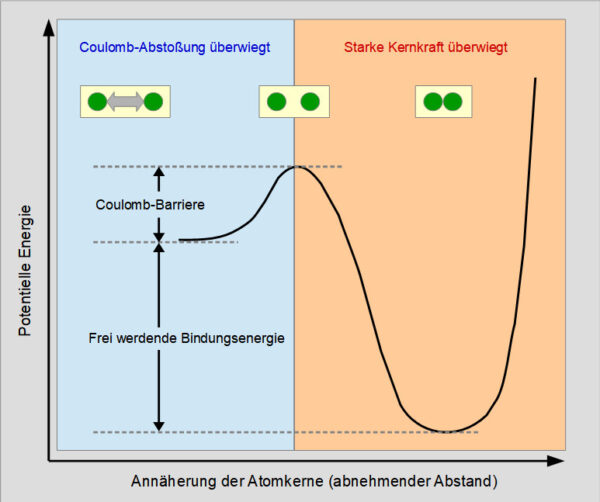
\includegraphics[width=0.5\textwidth]{graphics/potentielleKernenergie.jpg} \\
	    		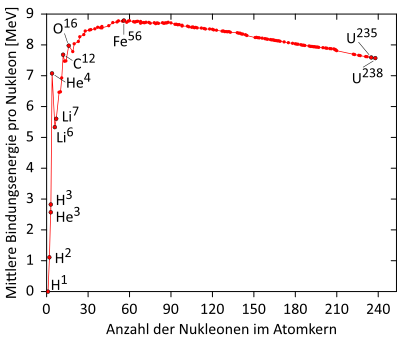
\includegraphics[width=0.5\textwidth]{graphics/bindungsEnergie.png}
	    		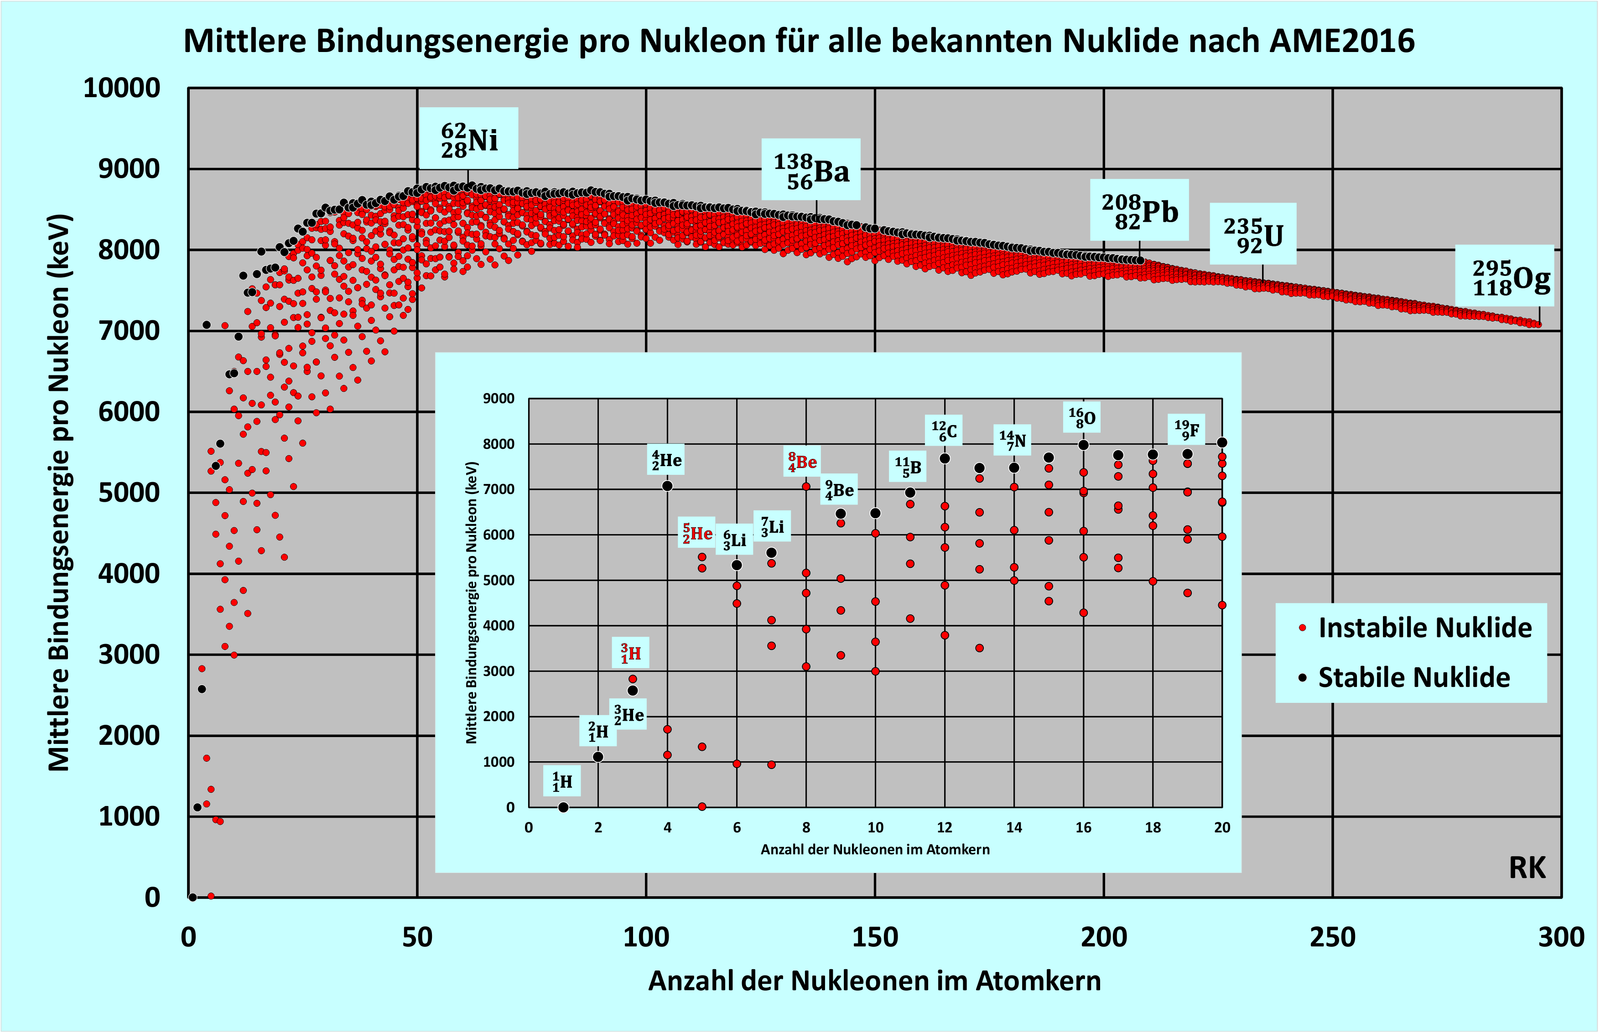
\includegraphics[width=0.5\textwidth]{graphics/bindungsEnergie_big.png} \\
	    		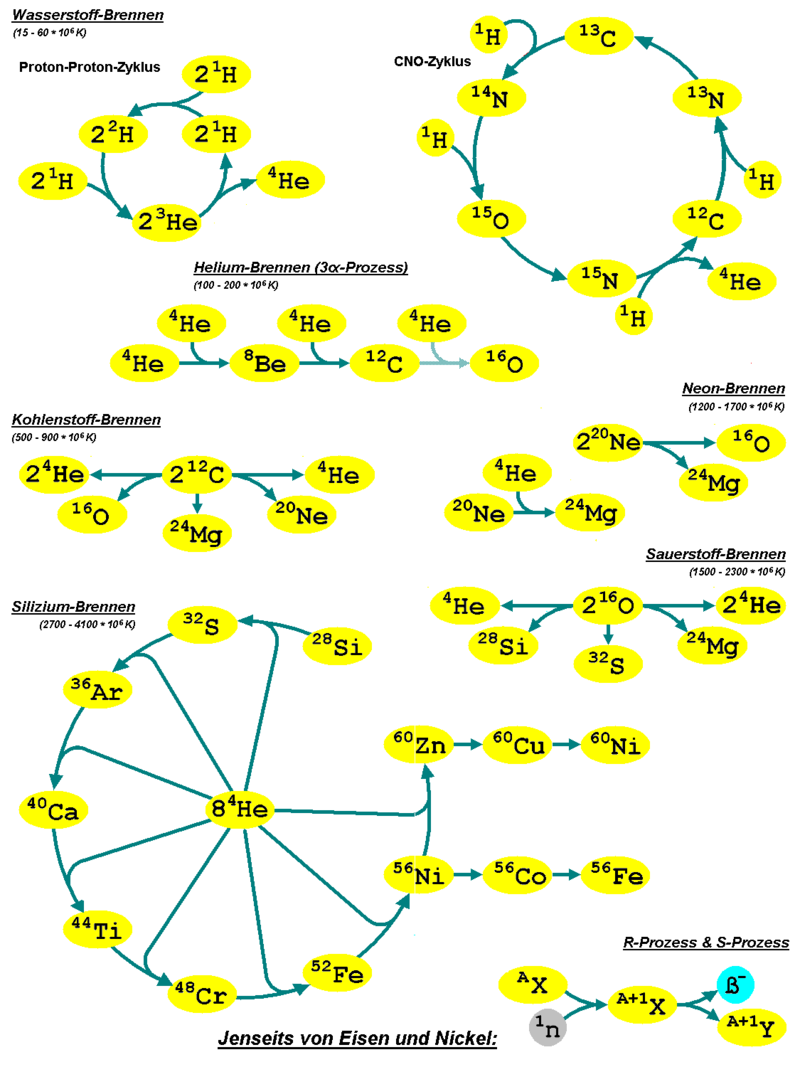
\includegraphics[width=1\textwidth]{graphics/sternzyklus.png} \\
	    		In den oberen Graphiken sieht man eine Visualisierung des Kernbindungsprozess, die Bindungsenergien einzelner Elemente und
	    		den Fusions- und Fissionskreislauf in Sternen. Zur Berechnung der Bindungsenergien muss $ E=\Delta mc^2 $ verwendet werden.
	    		Dazu wird der Massendefekt genutzt, wie bei der Fissionsenergie auch: $\Delta m = m_{Kern_{neu}} - (m_{Kern1} + m_{Kern2})$.
	    		Am Beispiel von der Fusion von Deuterium und Tritium: 
	    		
	    	\subsubsection{Einheiten für Radioaktive Strahlung}
	    		
	    		Mehr unter \href{https://gcm.schule/material/2024/physik/lk13/q4_wopla-05.md}{gcm.schule/material}
	    		
	    		\begin{tabular}{ |p{4cm}|p{1cm}|p{3cm}|p{4cm}|p{4cm}|  }
	    			\hline
	    			\multicolumn{5}{|c|}{\textbf{Einheiten}} \\
	    			\hline
	    			Bezeichnung & Symbol & Formel/Berechnung & Beschreibung/Kommentar & Grenzwerte \\
	    			\hline
	    			Halbwertszeit   & $ T_{1/2} [s] $   & \[ T_{1/2}=\frac{ln(2)}{\lambda} \] \[N=N_0 \cdot e^{-\lambda t}\] &   Zeit bis die Hälfte einer Ausgangsmenge eines bestimmten Isotops zerfallen ist. & Nicht behandelt. \\
	    			\hline
	    			Aktivität & A[Bq] &   \[A=A_0 \cdot e^{-\lambda t}\] \[\frac{\Delta N}{\Delta t}\]  & Anzahl der Zerfälle pro Zeit.   & Nicht behandelt. \\
	    			\hline
	    			Energiedosis & D[Gy] & \[D=\frac{E}{m}\] &  Strahlungsmenge, die ein organischer Körper aufnimmt. & Tod: 6Gy (in kurzer Zeit auf ganzen Körper)\\
	    			\hline
	    			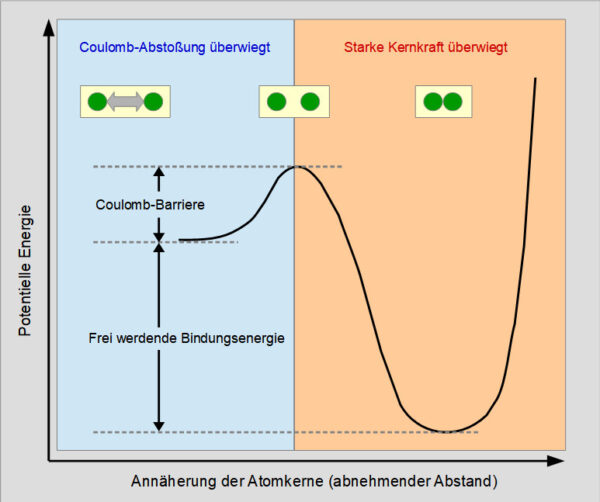
\includegraphics[width=0.5\textwidth]{graphics/potentielleKernenergie.jpg} \\
	    			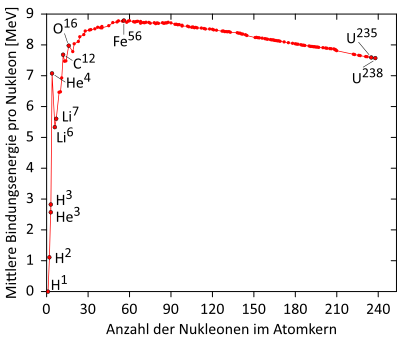
\includegraphics[width=0.5\textwidth]{graphics/bindungsEnergie.png}
	    			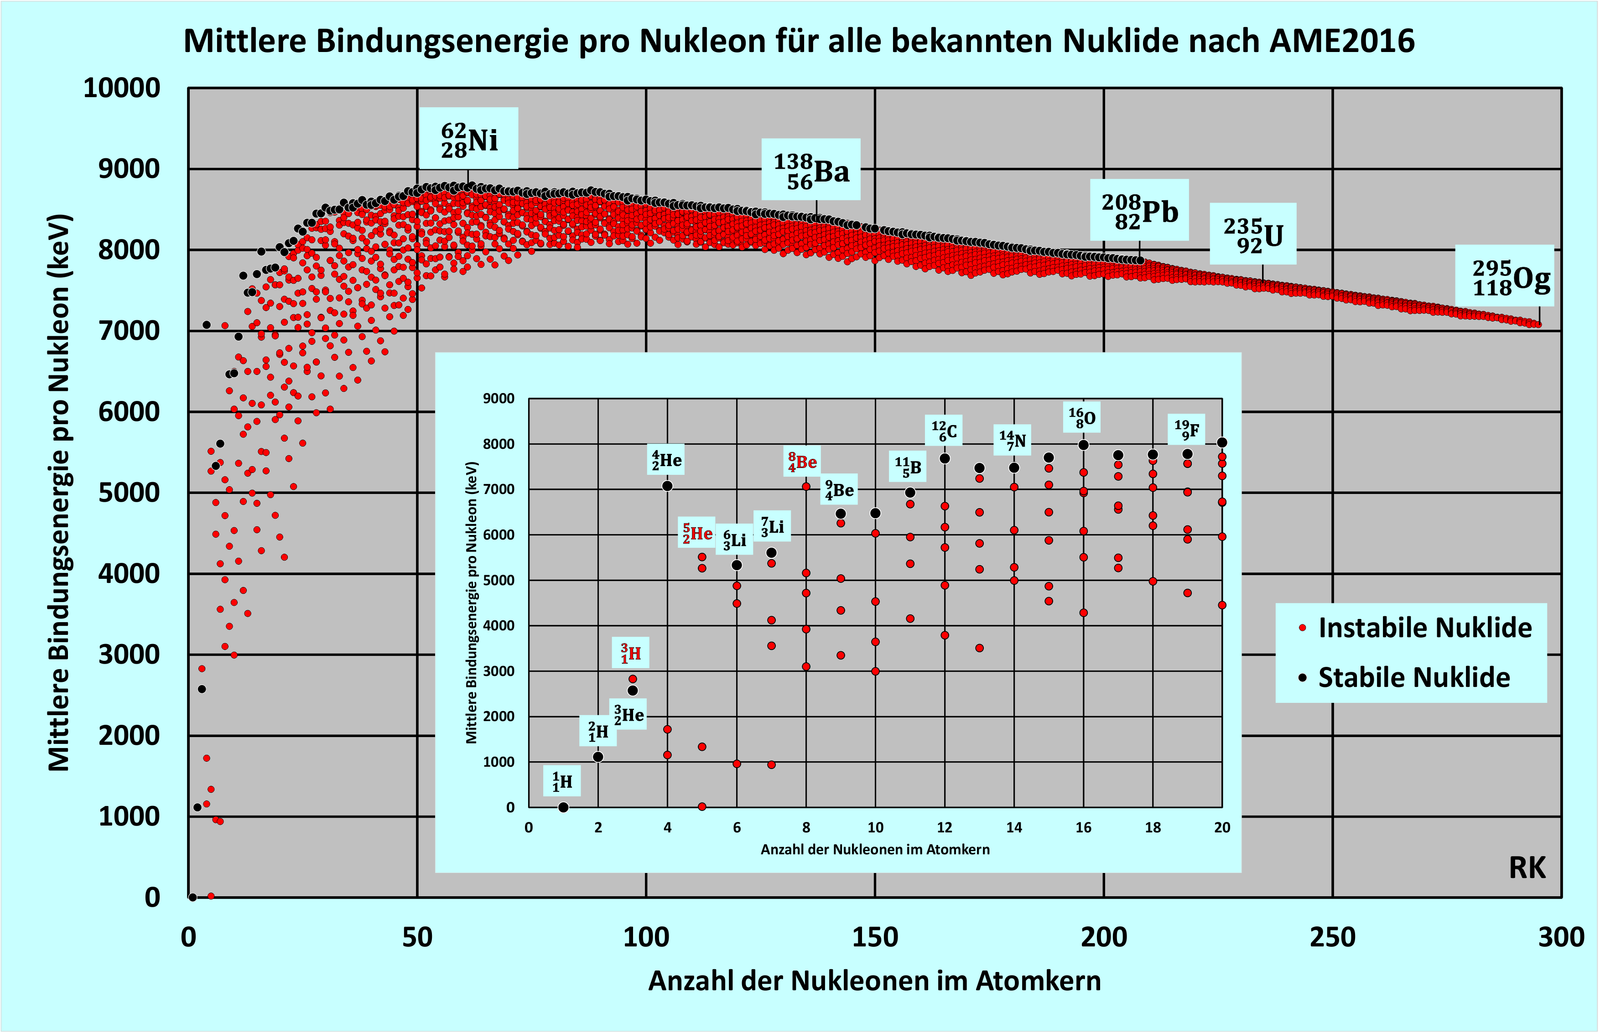
\includegraphics[width=0.5\textwidth]{graphics/bindungsEnergie_big.png} \\
	    			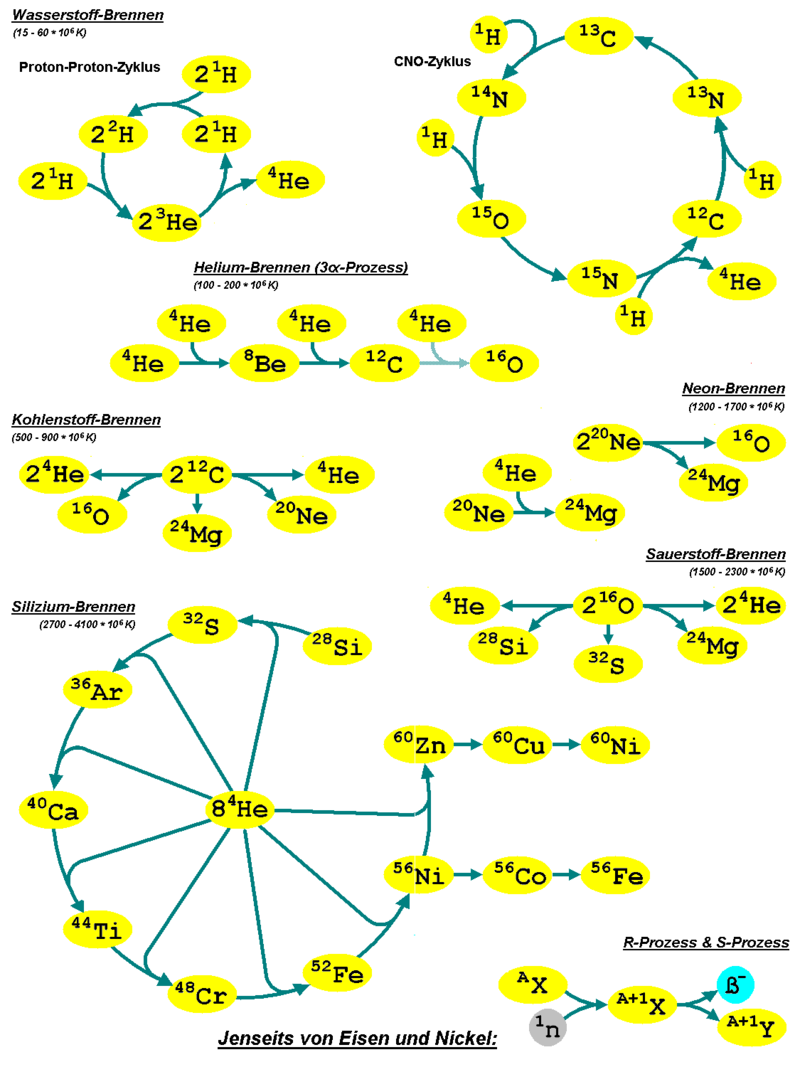
\includegraphics[width=1\textwidth]{graphics/sternzyklus.png} \\
	    			In den oberen Graphiken sieht man eine Visualisierung des Kernbindungsprozess, die Bindungsenergien einzelner Elemente und
	    			den Fusions- und Fissionskreislauf in Sternen. Zur Berechnung der Bindungsenergien muss $ E=\Delta mc^2 $ verwendet werden.
	    			Dazu wird der Massendefekt genutzt, wie bei der Fissionsenergie auch: $\Delta m = m_{Kern_{neu}} - (m_{Kern1} + m_{Kern2})$.
	    			Am Beispiel von der Fusion von Deuterium und Tritium:      Äquivalentdosis & $D_q$[Sv]& \[ D_q = D \cdot q \] \[q_{\alpha}=20\] \[q_{\beta}=1\]\[q_{\gamma}=1\] \[q_{N}=[2;10]\] & Energiedosis unter Berücksichtigung auf biologische Wirkung und Strahlungsart \[D_{q,eff}=D_q \cdot W_e\] $W_e$=Wichtungsfaktor & 250 mSv führt zu Schäden, 5Sv führt zum Tod (in kurzer Zeit) \\
	    			\hline
	    		\end{tabular}
    	
    	\subsection{Termschamata für Kernumwandlung}

        Mehr unter \href{https://gcm.schule/material/2024/physik/lk13/}{gcm.schule/material}

      


\end{document}




